%\addbibresource{../../Bibliography/bib_zotero20171106}

%\chapter{Mechanistic model for plant community dynamics centred around carbon allocation}
%Paper 1:
%\section{Introduction}

\begin{fullwidth}
The objective of this chapter is to develop the core concepts of the model, introduced in previous chapter, and explain the structure and design choices made during the model development. The first part focuses on the general context of alpine grasslands and some coexistence mechanisms at stake. The following part details the definition of the strategy space and the modelling of phenotypic plasticity, while introducing the key concepts of species memory and individual experience. Finally, the last part is a detailed description of the model following Grimm recommendations \cite{grimm_standard_2006}.
\end{fullwidth}

\chapter{Alpine environment: conditions, resources and perturbations}
\section{The scale of alpine grasslands}

\paragraph{The scale}
The scale is a determinant variable in the quantification of mechanisms that structure ecological communities \cite{bello_hierarchical_2013}, and therefor in modelling approaches. It is chosen based on structures that the modeller intends to explore, and determine the upper limit of mechanisms the model can reproduce. Large scales will favour geo-climatic and dispersal effects \cite{kleidon_global_2000} while small scales will focus on direct plant interactions processes or resource heterogeneity \cite{ soussana_gemini:_2012, maire_plasticity_2013, taubert_modelling_2014}. This is true for spatial scale, but also temporal scales. Because of ...reasons... , spatial and temporal scales are often correlated.

\paragraph{The resolution} The resolution is also determined by processes of interest and the scale of the model. 

\paragraph{Complexity: scale and resolution}

\section{Resources: light and water}
As mentioned in the previous chapter, resource fluctuations, heterogeneity and competition are important factors for coexistence. Unlike animals, plant mainly compete for the same resources: light, water and nutrients. Light is the source of energy that allow the transformation of inorganic carbon into organic matter through photosynthesis. Water has multiple function in plants: transport, structural support, and oxygen supply for photosynthesis. Nutrients are used in construction of cells and cell walls, and especially the production of proteins that act as cell machinery.

\section{Perturbations: frost, grazing and mowing}

\chapter{Multi-dimensional strategy space, carbon pools and trade-offs}
\section{Multi-dimensional strategy space and allocation pools}
%Leaf economic spectrum + Shipley + Poorter
%
%\subsection{Allocation or anatomy: a choice to make}
%what is SLA and SRL: cost of exchange area: tissue density, tissue thickness. Poorter 2009, grace2017, Katabuchi 2017, de la riva 2016\\
%THere is not only coordination -> part of RSR is explained by SRL:SLA\cite{freschet_explaining_2015}. Multiple source of information (memory) that affects these traits: composite traits that affect multiple fitness dimension -> memory not only for climate. -> but also coordination. More tight trade-off for root with smaller changes in SRL and more changes in RMF, the opposite for SLA. Need for a model that allow such asymmetry. 
%\cite{freschet_integrated_2015}
%\\

\subsection{The strategy space in \model}

\paragraph{What is a strategy space}
In an ecological agent-based simulation model a species will be defined by its values for the species specific parameters. They can be estimated from experimental data \cite{taubert_modelling_2014, maire_traits_2009,lohier_explaining_2014} or be picked from a strategy axis \cite{reineking_environmental_2006, kleidon_global_2000} composing a strategy space \cite{westoby_leaf-height-seed_1998}. The diversity of the species pool will depend on the number of values for each of these specific parameters, or traits, and the number of these traits. Each trait increasing the dimension of the strategy space \cite{laughlin_intrinsic_2014}. The ambition of this model being to simulated rich plant communities, the definition of these axis is crucial. Trade-offs between traits are excellent applicants for these specific parameters as they reduce the dimensionality of phenotypes to a small number of dimensions \cite{wright_worldwide_2004, diaz_global_2016, reich_world-wide_2014} while keeping the information of traits needed to describe the plant functioning. Trade-offs emerge from ecological and physical or biological constrains, by considering these constrains Darwinian demons are avoided.\\

While considering too many axis does not improve community description, a certain number is needed to have strategic diversity \cite{laughlin_intrinsic_2014}. This is intuitively explained by the fact that each trade-off is closely related to a particular aspect of fitness or mechanism for coexistence (\textit{e.g.} reproduction, competitve ability, resistance to resource shortage, predation, etc.). In this model, multiple aspects of plant life are represented: germination with the germination rate for storage effect \cite{chesson_general_2000, adler_climate_2006}, dispersion with seed mass \cite{westoby_leaf-height-seed_1998} or tissue construction cost \cite{reich_leaf_1992, wright_worldwide_2004, reich_world-wide_2014}. Main components of plant growth and life history are covered by such trade-offs and driven by mechanisms shared by all vegetation systems. Because of that, the model has a great potential of genericity and diversity. It can be easily adapted to other plant communities with specific calibration, and extended with couples of biological process and differenciation axis (\textit{e.g.} root herbivory and associated resistance carbon pool). The the trade-offs used in the model are detailed in the model description below \sidenote{see serction \ref{chapter:model-description}.}. These axis should, in such models, be independent, (\textit{i.e.} it is physically and biologically possible for a plant to take any position in the space drawn by two given axis) and result from physical or biological laws (ensuring that impossible strategies are indeed excluded from the model). First, it is a condition for parsimony of the model. Second and more interesting reason is that any trade-off emerging from the model should have an ecological interpretation \cite{maire_disentangling_2013}. \\
 

One way of constraining plant strategies to certain axis is to consider allocation trade-offs \cite{kleidon_global_2000, reineking_environmental_2006}. An allocation trade-off is the translation of the mass conservation rule that prevents the allocation of biomass to distinct carbon pools. If biological functions are related to organic matter pools (photosynthesis to leaves, water and nutrient uptake to roots), then the sum of biomass to invest in each carbon pool (therefore in each function) cannot exceed the total available biomass: leaving the plant with a choice on the balance between the different functions. Allocation trade-offs have the advantage to be easily implemented and be intuitive. By design, a partitioning factor value corresponds to a position on the related strategic axis. In \model, five main trade-offs are captured by allocation trade-off: (1) development vs reproduction: partitioning factor between reproduction and maintenance of vegetative tissues (when plant is mature), (2)  persistence vs dispersion: partitioning of reproduction biomass between persistence (storage) and production of new propagules (seed/clone production), (3)aboveground vs belowground competition: investment between shoot and root, \cite{kleidon_global_2000, reineking_environmental_2006, taubert_modelling_2014}(4) slow vs fast: construction cost trade-offs between active and structural tissues in both shoot and root and (5) growth vs resistance: partitioning between stored biomass and frost resistance carbohydrates \cite{cai_changes_2004}. This last trade-off can be extended to other carbon pools of specific resistances, for example to herbivory. Modification of these coefficient during life history is a way to introduce plasticity in the model. The rules driving such changes for some of this partitioning parameters are described in the following section.\\


One of these trade-offs, (4), is key and related the construction cost of organs (independently leaves and roots). Highlighted at global scale and for leaves, the Leaf Economic Spectrum \cite{wright_worldwide_2004} draws an strategic differentiation axis from conservative slow species and exploitive fast species. The construction cost has long been identify as a factor of strategic differentiation in plant communities\cite{westoby_leaf-height-seed_1998}. This strategic axis, being related to many functional traits: SLA, LDMC, LNC, leaf longevity, Amass, etc.\cite{wright_worldwide_2004} is of crucial importance. First, these traits are closely related to the characterisation of plant communities and the assessment of services \cite{grime_benefits_1998}. Second strong links and correlations can be made between these soft traits physiological traits \cite{craine_functional_2002, reich_variation_2003, wright_worlwide_2004}. Finally, a species resource use strategy is closely related to its responses and vulnerability to changing conditions \cite{poorter_causes_2009, dwyer_specific_2014, deleglise_drought-induced_2015}. The traits related to this trade-off play a major role both in individual growth and physiology, and in community services and response to gradient. Therefore it is essential to the model. Questioning the underlying mechanisms for such strong trade-off is necessary to implement satisfying representation in the model.\\

\textbf{Change this: may be start with shipley results, then composite stuff. Question: should it be here, or in the following part ?}

These trade-offs between highly productive tissues with low construction cost and short lifespan called exploitative, and more conservative strategy with longer lifespan but lower productivity are mainly observed thanks to soft traits such as SLA for LNC \cite{wright_worldwide_2004}. Mechanistic model require traits related to physiology and organ performance \cite{soussana_gemini:_2012, lohier_explaining_2014}, but link can generally be done between these traits and soft traits. However traits such as SRL or SLA are composite traits emerging from different organ properties \cite{ryser_importance_1996,john_anatomical_2017}, where tissue density and organ thickness are the main determinants. "\textit{A necessary trade-off between allocation to structural tissues versus liquid phase processes}" has been identified by Shipley et al. \cite{shipley_fundamental_2006} as one of the two main factors for the leaf economic spectrum to emerge. Such allocation trade-off can indeed explain differences in construction cost as the liquid phase corresponding to the "active" part of plant tissue, the cell content, have much lower dry volumetric mass than its "structural" counterpart, the cell-wall. Also active tissues containing the protein machinery for photosynthesis and water absorption, a higher proportion of high protein concentration tissue would be correlated to higher nitrogen concentration in the organ on the "fast-slow" spectrum, along with a higher mass-based photosynthetic rate \cite{reich_world-wide_2014}. On the other end, the structural tissues give the organ a higher lifespan \cite{mediavilla_internal_2001, ryser_importance_1996} that compensate for lower productivity \cite{westoby_time_2000}. Such trade-off can be apply to both shoot and roots \cite{craine_functional_2002, tjoelker_linking_2005, reich_world-wide_2014}. From that, the decomposition of organs between active and structural tissues constitutes a strong basis to model construction cost trade-offs as the main parts of the global strategy space.\\

The Similar axis of differentitaion has been demonstrated for roots \cite{ reich_world-wide_2014, tjoelker_linking_2015}. The necessity for independent similar axis for leaves and root can be discussed with respect to coordination between shoot and root activities. Because perfect equilibrium cannot be guaranteed in all conditions, strict coordination cannot taken as a principle for the reduction of strategy space. Moreover, empirical results suggest small deviations from coordination are common \cite{freschet_explaining_2015}. The leaf economic spectrum being conserved at the intra-specific level \cite{ hu_novel_2015} is another reason to include such trade-of as it would be a good basis for phenotypic plasticity \cite{freschet_plasticity_2013}.\\


%Take home message ####################################
\textbf{The use of allocation trade-offs allows the construction of a generic multi-dimensional strategy space where a high diversity of species can potentially coexist. Because this space is based on physic laws, it ensures the non existence of Darwinian demons and does not limit the species or individual plants to tested parameters and strategies. To be complete the link between carbon pool allocation and physiology must be determined within the respect of similar biological or physical laws.}

\section{Craft a trade-off: active and structural tissues}

Allocation trade-offs offer great flexibility and are easily understood and implemented. However, when they control the value of traits (SLA or SRL) involved in multiple processes, a balance must be found to avoid that: (1) one process is ignored because has a low relative importance on fitness (becoming useless to the model), (2) the effects of processes involved show strong response curves to the allocation and there is only one global\sidenote{I use the term global here to designate the multidimensional space draw by the axis of interest and other variables play a role in involved process (e.g. resource availability, temperature etc...).} optimum. The idea behind a trade-off is that multiple positions are viable in different conditions or in association with other strategies. The leaf-economic spectrum, in addition to rely on the active-structural tissue trade-off, also requires "\textit{an evolutionary trade-off
between leaf photosynthetic rates, construction costs, and leaf longevity}". This trade-off is explore in this section of the document.\\

In the framework of the model, plants share the same global parameters, and the maximum photosynthetic rate should be the same. Because photosynthesis relies on the exchange of gases ($CO_2$, $O_2$ and $H_2O$) and the interception of light, it is related to exchange area. Considering one shared parameter for maximum area-based potential exchange rate satisfy both the need for a shared parameter and a way for plant to vary their mass based exchange rate by changing its proportion of active tissues. This is in agreement with the LES that describe strong relationship between mass based traits and limited ones for area-based variables \cite{wright_worldwide_2004}, and explain the first part of the trade-off between photosynthetic rate and construction cost. The second part is the relationship with the longevity. The longevity is often correlated to SLA in empirical studies, however this is mainly explained by differences in tissue density and toughness than in thickness (other component of SLA) \cite{}. For this reason we can directly link the leaf longevity to active tissue proportion. Respiration is also increased by the increase of proportion of photosynthetic tissues \cite{kleidon, reich}. We have now a trade-off between a gain function (exchange area gain by changes in densities) and a cost function (tissue turn over and respiration). This should be enough to explain different strategies \cite{westoby}. However the model need internal limits to avoid the gain function to lead to only active tissue organ (or only structural). These limits are required to allow individuals or species to change position along these axis (plasticity or strategic shift). The convex shape of gain function in association with a minimal cost (minimum turn-over cost above maximum potential gain) is enough to limit the allocation to structural tissues only. To avoid allocation to only active tissue, that would correspond to an organ made of protoplasts, the cost function need higher than the potential gain. To acheive that an ... function is chosen. This choice ensure that the potential gain function has an optimum different from the borders. \textbf{(see figure)}.\\

\paragraph{gain as function of conditions}
Active got closer to optimum, but less active and positive gain in more conditions. Can I demonstrate this with formulas ? (gain = function(condition))
\\

The potential gain is not only function of active tissue proportion, but also depends on resource availability. Changes in resource level imply changes in slope of gain function and a shift of the organ optimum for tissue allocation. This shift make more conservative strategies more interesting when resources are scarce, while more exploitative allocation strategies are better for high resource availability. This link between optimum allocation and resource level could be used to define the best phenotype according to experience conditions, but the organ strategy cannot be disconnected from the whole plant strategy and allocation.\\

The phenotype (within the subspace of vegetative allocation) depends both on the individual efficiency of organs and the balance between shoot and root activity. This balance, often used to model plant plastic allocation and considered between light and nitrogen \cite{lohier, soussana}. In the context of mountain grasslands and global change, the water... The integration of nitrogen as a limiting solution is discussed in latter chapter. The balance between shoot and root activity being key in overall performance, the root shoot ratio (RSR) will be determined as a function of estimated availability.

% There you have to sell your memory stuff !

\subsection{Species memory and phenotype determination}\label{subsection:memory}

\paragraph{Memory of species: a driving trait}

phenotype = ensemble of response trait values. Emerge from default trait + environment.\\
Composite traits are defined by the interaction of different, independent, driving traits. What is a driving traits ? Biology: genetic information. This genetic information is selected by climatic conditions. If we can make a link between optimum value for a trait and environmental conditions, then store external conditions and use link between.\\


%Th example of the leaf trade-off and the importance of resource availability for optimum position.\\


%The coordination and the difficulty to define a phenotype\\


%Take home message ####################################
\textbf{The decomposition of organs organic matter in active and structural carbon pools makes a link between allocation and physiology and draws a subspace within the strategy space where individuals can move and change their phenotype. Limiting mechanisms restraint the viable options to realistic values along these axis. Within this space, the resource availability and external conditions play a major role in the expression of the strategy.\\ %not convinced by this last part.
}


%Chapter take home message ####################################
\textbf{Flexible, allocation based, diversity and movement}

\chapter{Modelling phenotypic plasticity}


\section{Plasticity as a strategy: between species memory and individual experience}

\subsection{Concept of active plasticity as a strategy}
\paragraph{Decomposition of plastic response}
Active plastic response is highly integrated and involve a lot of regulatory processes. It is impossible to represent all regulatory processes involved in an APR (because of our lack of knowledge and their complexicity). Alternatively, the concept of \textit{integrated response} can be conceptualised. It supposes link, or coordination, between the experienced conditions and the phenotypic response. This can be translated, in the model framework, by the existence of explicit link between a representation of external conditions and a phenotype matching this conditions: the \textemph{allocation rule}\sidenote{the use of the word \textit{allocation} is justified here since the phenotypic plasticity in \model is reduced to changes in allocation.}. Another key work is \textit{anticipatory}. It supposes that the plant knows, or at least have an idea of the future conditions. This is really the point of an active plastic response: change the phenotype to better match future conditions. A representation of future is also called a \textemph{projection}. The projection and the allocation rule together form the active plastic response.\\
If allocation rule is not obvious and is discussed latter\sidenote{see paragraph \ref{section:allocation-rule}}, the idea of projection is fairly intuitive. The projection will correspond to a value for a given metric that represent the external conditions. It can be resource availability level, temperature, herbivory risk, etc... If such metrics can be given at the community scale, it make sense to use plant centred measure of these variables for two reasons: (1) take into account the spatial heterogeneity, (2) plant experience of conditions is necessarily egocentric. The details on how experienced conditions are interpreted by plants in \model is described in section \ref{chapter:model-description}.

\paragraph{Control of plasticity}
Active plasticity is now represented by a projection and allocation rule. However, how a species can control the whole process is unclear. In theory both projection and allocation rule can species specific. In nature plants generally have structurally similar regulatory processes\sidenote{see box \ref{box:molecular-basis}.} and response to external stimuli is translated (and stored temporarly) thanks to the accumulation of chemical compounds\cite{need-references}. These mechanisms suggest that, while the allocation rules are mainly  shared, individuals vary on the information level (i.e. concentration of phyto-hormones), or in the context of the model: plant vary in projection. This control  of active plasticity is supported by the model design. The number of rules that can drive the allocation is reduced and discrete, while the projection is multi-dimensional (one dimension per external variable considered), continuous and high flexible with a reduce number of parameters\sidenote{details in paragraph \textit{estimation of conditions} in section \ref{chapter:model-description}.}.
For this reason \textemph{projection} is chosen to be the \textemph{controlling factor} of active plasticity, while the allocation rule is \textemph{fixed} and \textemph{shared} between all species. Therefore an individual with fixed projection wont be actively plastic, despite the fact that it could express apparent plasticity because of external factors: reduced resource availability, grazing, frost damage, etc... The model has now a concept for active plastic response\sidenote{In the rest of the document terms \textit{plasticity} or \textit{phenotypic plasticity} will refer to \textit{active plastic response}.} controlled by the projection of external condition. The next question that need to be answered is: how do species differ in their plastic response ?\\


\paragraph{Species specific plasticity}
In \model, the projection of external conditions is the mean for plants to alter their phenotype in response to changes in experienced conditions. Since the allocation (or driving) rule is shared by all plants, if the projection of external conditions is also shared by all plants, then is the response still active plasticity ? The first intuitive answer is \textit{yes}, since the conceptual framework is respected and plants would react to changes in conditions that would affect the projection. But, such response would be equivalent to a direct external control of the climate on the phenotype. In such case, species would not have control on how the phenotype varies, that would be fully controlled by shared projection and shared allocation rule. This is passice plasticity. To have proper active plasticity, the species need to be able to \textemph{regulate} the plastic response. If species can regulate plastic response thanks to species specific parameters, plasticity becomes a \textemph{strategy}. This is in agreement with Bradshaw vision of phenotypic plasticity as a trait, or a character, subject to selection and evolutionary processes\cite{bradshaw_evolutionary_1965, bradshaw_unravelling_2006}. How do species regulate plastic response to make it a strategy?\\

\textbf{Plasticity}: expected environment -> phenotype, here phneotype is equivalent to biomass partitioning, that means expected environement -> allocation coefficients. Then memory -> expectations -> allocation. Because low dimensions, and we want diversity, and the link between memory and allocation might not be a function (one memroy give exactly one optimum allocation), in the model this relationship is not verified. Species specfic traits are used to allow for different strategies to be associated to a same memory (different plants won't have the same strat, despite sharing the projection)\\
%Once the plasticity is introduced, talk about the memory. Now you can also talk about the mapping/consistency between both and the difficulties to use both.


\subsection{Projection of external conditions: between species memory and individual experience}

\paragraph{Build a projection}
The projection is the way plant controls phenotypic plasticity. A projection is an idea of the future based on available information and understanding of phenomenon. Ones could discuss what is the understanding of the climate by plants, while others can focus on how to represent such understanding and state that fine molecular regulatory processes can reproduce and store such information. The focus is on the construction of the projection with respect to the different sources of information a plant has: (1) its experience of climate and external factors, and (2) its ancestors memory\sidenote{see paragraph \ref{subsection:memory}.}.\\
While, for any given individual plant, the experience of external conditions varies in time, the memory stays fixed. There is a clear contrast between variable experience of conditions and the fixed species memory. A way to represent different strategies and the level of control the plant apply on projection is to vary, between species, the relative weight of species memory against individual perception. This species specific parameter, the \textemph{confidence in species memory}, sets the \textemph{stability} of the projection with respect to individual experience. The capacity to adapt the phenotype to changing conditions is directly linked to the projection changes. High confidence in species memory translates in low amplitude of projection variations, and though in low active plasticity.\\
The calculation of projected resource availability levels, or temperatures, are detailed in dedicated paragraph of the model description. The key message is that the species has control on plasticity with both its confidence in species memory, and the said memory that alters the projection. The relative impact of memory and confidence is described in figure \ref{fig:memory-confidence}.

% The species specific memory of external condition has been described\sidenote{paragraph \ref{subsection:memory}} as a way to match certain traits (mainly root:shoot ratio) with external conditions. The memory is a metric of resource availability that is used to partly (potentially entirely) determine the phenotype of plants.

\paragraph{The paradox of plasticity}

While the representation of plasticity as a strategy increases both model species diversity and potential  diversity of response \cite{ ryser_consequences_2000, kichenin_contrasting_2013}, plasticity itself may reduce plasticity. Indeed, plasticity lead to a change in phenotype in response to condition changes, while this phenotypic change is unlikly to be identical, its direction will probably be similar. Few mechanisms can prevent convergence of phenotype besides the diversity in memory and plasitcity: (1) changes in competitve hierarchy may lead to differences in individual experience of conditions, (2) specificity of the external driver, e.g. selective herbivory of more digest species, (3) relative position of the optimum phenotype.\\



Or can a plant be plastic and unique ? The paradox of plasticity and diversity.\\
Plastic will neceseraly reduce the space (as there is convergence, unless different strategies of adaptation).\\

 Because the plasticity is a strategy and not a default behaviour, its effects on individual performance have to be tested. But it also opens a lot of interesting questions around the costs and benefits of plasticity, and the co-selection with the resource use strategy.\\
Moreover this particular implementation of plasticity limits risks of convergence while allowing plants to evolve in the strategy space defined earlier.

\subsection{On the difficulty to match strategy and conditions.}

 
 
%Take home message ####################################
\textbf{The projection of external conditions, driving the plastic allocation of organic matter, lies on a balance between species memory and individual experience. Its design make of plasticity an axis of strategic differentiation alongside the other strategy axis. Thanks to this innovative design, the model can be used to examine the ecological relevance of plasticity in different conditions and in association with different strategies. The effect of allocation rules and projection stability can be explore independently or conjointly for a better understanding of relative importance of allocation and plasticity.}
% It is possible to explore independently or conjointly the effect of allocation rules and projection stability on individual and community dynamics.


\section{Driving rules of allocation}\label{section:allocation-rule}

Allocation rules is determinant in the model behaviour as it is shared by all species, and link the projection of conditions with the phenotype. Multiple options are possible to drive plasticity, but they can be divided in two main categories: (1) determining, (2) directive. Function from the first category fully determine the phenotype (within the plastic strategy space), while functions from the latter group direct the phenotype toward a sub-space and other parameters are needed to determine the exact new phenotype.\\
The two type of rules have different strengths and weaknesses that are detailed in table \ref{table:allocation-rule}

\begin{table*}
\caption{Two types of allocation rules: strengths and weaknesses} 
\label{table:state_var_plant}
\begin{center}%
\begin{tabular}{l c r}
Strength or weakness & Determining & Directive \\ 
\hline 
Phenotype fully determined & \textcolor{myGreen}{$\bullet$} & $\circ$ \\
Risk of convergence & $\bullet$ &  $\circ$ \\
Reduction of functional diversity & $\bullet$ &  $\circ$\\
Discrepancy between parameters $\bullet$ &  $\circ$\\
Strong plasticity effect & \textcolor{myGreen}{$\bullet$} & $\circ$
\end{tabular} 
\end{center}
\vspace*{0.5cm}
\end{table*}

%Take home message ####################################
\textbf{... few words on the space ?\\
The driving rule of plasticity defines whether or not the choice of the  phenotype is fully determined by the projection of external conditions or constrained by some species specific parameters. The effect of this balance between projection and parameters is crucial in the model behaviour. In any case the projection is the main control on individual plastic response to change in conditions, offering possibilities to modulate individual plasticity despite a shared mechanism.}




\chapter{ODD description of the model \model}\label{chapter:model-description}



\begin{fullwidth}
%\begin{abstract} 
\noindent
This document is a detailed description of the \model model. This description is based on the ODD protocol of Grimm et al. The model is inspired by multiple other forest and grassland models (for grassland models see particularly Taubert \parencite{taubert_modelling_2014} and Lohier \parencite{lohier_explaining_2014}). It differentiates itself from these models by the incorporation of phenotypic plasticity in a generalizing framework for plant functioning. This allows it to be used to both to explore the fundamental effects of phenotypic plasticity the dynamics of rich grass communities and the impact of the phenotypic plasticity on plant interactions. The general approach and the practical details are further detailed in this document.
%\end{abstract}
\end{fullwidth}



\section{Model overview}

\subsection{Model purpose}

The development of \model is motivated by the need for a flexible tool to explore the complex dynamics of mountain grassland communities, in the context of global change. This tool should, by a better understanding of community dynamics and representation of plant strategies and interaction, also help in the assessment of ecosystem services in new conditions. We believe that to capture the dynamic of such communities, we need to understand and represent first the individual response of plants to fluctuating levels of resources, and the impact of plants on the resources. Individual responses and relative impact should follow general rules of plant physiology but also integrates specific behaviour based on the species resource use strategy and individual characteristics. Therefore the model should allow following distinct individuals from different groups (e.g. species) in a spatially explicit environment where they compete for resources.\\
\indent Moreover, since we focus on the community levels, coexistence mechanisms are important and we should include a certain number of these if we want to maintain diversity to observed levels. These mechanisms include: multiple resources competition (water and light), spatial and temporal heterogeneity of resource levels, strategic trade-off between species, perturbation mechanisms (frost, management), link  to meta-population, etc...\\
\indent The model is built to try to satisfy conditions to reproduce and explore mountain grassland community dynamics. In the current version of the model (\version), a generalist approach has been privileged, and focus on some coexistence maintenance mechanisms and integration of phenotypic plasticity framework. In this state, the model has to be seen as a toy model with good generalisation potential. The link between to ecosystem services are not included, but we can easily imagine to compute them from the community trait distribution. All processes and mechanism are detailed below.

\begin{figure}
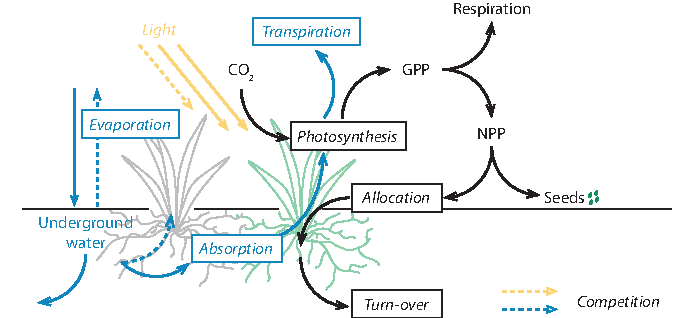
\includegraphics[width = 1\linewidth]{./1_Introduction/graphics/model_cycles.pdf}
\caption{Model overview. \textcolor{myBlue}{Water} and \textbf{carbon} cycles are represented. Processes are represented framed and in \textit{italic} by contrast with pools that are not framed and in regular fontface. Dashed arrows indicate loss of resource (for the \textcolor{myGreen}{focal plant}) due to competition.}\label{fig:overview}
\end{figure}


\subsection{State variables}

\paragraph{Scales}
In mountain grasslands individuals (tillers) generally do not grow big and interact only with close neighbours and form little patches. And thus it is possible to represent a rich community at a fairly small scale ($\approx$ dm or m), but the spatial resolution should be relatively fine ($\approx$ cm) to capture inter-individual interactions. Because the model is intended to explore climate change impact on mountain grasslands, it can run on multiple growth seasons separated by snow-covered periods, but must also integrate the intra-seasonal variations at daily scale. Mountain weather (mostly temperature) is known for its large hourly variations, it would, however, require too much computational power to consider such variations. In addition to this argument, we believe that even though they imply physiological flexibility and specific strategies for plants experiencing these conditions, they will not have a huge impact on overall community dynamics changes caused by the climate change. That why hourly variations will not be considered and physiological processes are estimated at the daily timescale.

\paragraph{Plants} The plants are described in the model by state variables described in table \ref{table:state_var_plant}. The best way to understand how plant are represented is to imagine two homogeneous cylinders on top of each other, the shoot cylinder varying in radius and height representing the light acquisition (and shading) zone, and the root cylinder varying only in diameter (because of shallow soil in mountain ecosystems) representing the water acquisition zone. These cylinders are centred on cells of the torus simulation plan.\\
\begin{marginfigure}
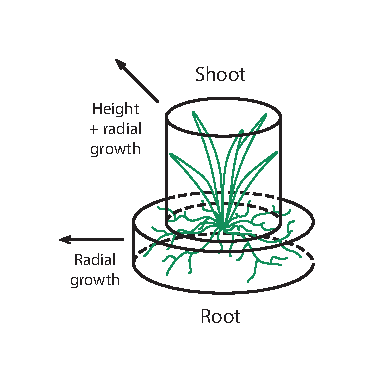
\includegraphics{./Figures/plant_geometry_m.pdf}
\caption{Plant geometry and growth axis.}
\end{marginfigure}
\indent In addition to classic variables (age, position, height, diameter, shoot and root biomasses) the plants are described by traits, that can be species-specific or non-specific, others are variable (SLA, SRL) and depend on particular traits that are unique to this model: the \textbf{ratio between active tissue and structural tissue} (in shoot and root) (variables $\frac{act}{str}_{ag}$ and $\frac{act}{str}_{bg}$ in table \ref{table:state_var_plant}). This couple of traits come from the evidence that numerous trade-off observed in leaves can be explained (at least partially) by this allocation trade-off between active tissue producing organic matter, but increasing respiration, and structural tissue that increase tissue lifespan.

%TAble of plant state variables
\begin{table2*}
\caption{State variables of individual plants} 
\label{table:state_var_plant}
%\begin{center}%
\begin{tabular}{l|l|c}
Variable & Description & Unit \\ 
\hline 
x & x position on the grid & cells \\
y & y position on the grid & cells \\
age & age & days \\
sp & species & - \\
$BM_{ag}$ & above-ground biomass & g \\
$BM_{ag_sen}$ & senescent above-ground biomass & g \\
$SLA_{sen}$ & senescent above-ground biomass & $cm^{2}.g^{-1}$ \\
$BM_{bg}$ & below-ground biomass & g \\
stem & stem biomass & g \\
$\frac{act}{str}_{ag}$ & above-ground active on structural biomass ratio & g/g \\
$\frac{act}{str}_{bg}$ & below-ground active on structural biomass ratio & g/g \\
h & height & cm \\
r & shoot radius & cm \\
r\_r & root radius & cm \\ 
$light_{exp}$ & above-ground potential resource availability & gH2O.leaf area\\
$water_{exp}$ & below-ground potential resource availability & gH2O.root area\\
\end{tabular} 
%\end{center}
\vspace*{0.5cm}
\end{table2*}

%little scheme to show what it looks like

\paragraph{Species} Plants are characterised by state variables that describe them individually, but they also share common characteristics with individuals of the same group, (we will refer as \textit{species} to talk about this group in the rest of the document even though it could be a group at another scale (i.e. population, clones). These species are the groups present in the meta-population and that can invade the simulated ecosystem. There are described by multiple traits characterising the strategy of the species (table \ref{table:state_var_species}).


%TAble of plant state variables
\begin{table2*}
\caption{Species traits}
\label{table:state_var_species}
\begin{center}
\begin{tabular}{l|c|c|l}
Trait & Range (close range) & unit & trade-off or strategy\\
\hline 
seed mass & (0.00001 - 0.001) & g & seed ouput vs seedling productivity\\
maturity & - & green biomass & flowering time vs reproduction potential\\
fract\_dev & 0-1 (0.05-0.6) & - & blooming vs persistence\\
fract\_rep & 0-1 (0-1) & - & reproduction vs persistence\\
geometric constant ($k_{g}$) & (0.1 - 20) & - & competition sensitivity vs self-shading\\
plasticity stability & 0-1  (0.8-1) & - & genetic information vs experience\\
initial water resource & (0.001 - 0.05) & $gH_{2}O.cm^{-2}$ & water resource niche\\
initial light resource & (0.001 - 0.05) & $gH_{2}O.cm^{-2}$ & light (in $H_{2}$ equivalent) resource niche\\
$\frac{act}{str}_{ag,d}$ & (0.03 - 0.3) & $g.g^{-1}$ & active vs structural tissue\\
$\frac{act}{str}_{gg,d}$ & (0.03 - 0.3) & $g.g^{-1}$ & active vs structural tissue\\
mean temp. & (0 - 5) & \celsius & early vs late germination\\
germination rate & 0-1 (0.5 - 1) & - & good season bet-hedging\\
thickness & 	(0.012 - 0.05) & cm & WUE vs light efficiency (not in this version)\\
\end{tabular} 
\end{center}
%\vspace*{0.5cm}
\end{table2*}
%table of species traits. trait, range, distribution, trade-off or strategy associated.

\paragraph{Seed-bank} The seed-bank is the transition state between the different seasons. Individuals may persist thanks to stored resources, but they can also reproduce by the production of new individuals. A lot of grasses use clonal reproduction, in addition, or replacement of sexual reproduction. This type of reproduction is characterised by a persistent link between the newly produced individuals and the parent one that allows the two to communicate and exchange resources. Such dynamics are complex and costly to represent as the link between ramets must be stored and strategies defined for the resource distribution (see Oborny 2012) for more details on clonal growth modelling). To avoid too much complexity, it is possible to approximate the representation of clones to big seeds with little dispersion around the parent plant\footnote{This would take advantage of dispersion kernels. Not implemented in the current version. Dispersion is uniformly random within the simulation plan}. For this reason, reproduction mechanism is reduced to sexual reproduction mechanism with the production of "seeds". Seeds are stored in the seed-bank and only defined by their species and positions. 

\paragraph{Soil}
\begin{marginfigure}
\includegraphics{./Figures/soil_section_m.pdf}
\caption{Soil section.}
\end{marginfigure}
The soil is an important aspect of the model as it drives (with the precipitations) the water competition between individuals. It is however limited, as in numerous vegetation models, to a grid characterised by its capacity to retain water, and its depth. Only the first component (water retention capacity) is spatially variable and is described by the critical water content (minimum soil water content), the saturation water content (maximum water content, the water non absorbed leaves the system we assume the same root depth for all species), and the current water content (temporally variable, depending on competition, precipitation and evaporation, between the critical and the saturation water content) only dynamic variable among the three.

%table of soil state variables

\subsection{Process overview and scheduling}

As mentioned the model runs at a daily step to capture individual responses to conditions and over multiple seasons to capture long temporal dynamics. Some processes occur (or are evaluated) at the daily time-step, some at the season time-step. The following ordered list presents the different processes and the scheduling over days and season of one simulation.\\
\indent One season can be divided into the following parts:
\begin{marginfigure}
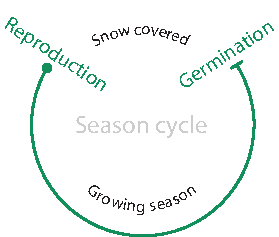
\includegraphics{./Figures/season_cycle_m.pdf}
\caption{Seasons cycle in \model.}
\end{marginfigure}
\begin{itemize}
\setlength\itemsep{0em}
\item \textit{germination}: marks the beginning of the season when the ground is no more snow-covered;
\item \textit{growing season}: consists in daily processes like competition, production of organic matter (OM), allocation, and death lottery;
\item \textit{reproduction-invasion-persistence}: marks the end of the season when the first persistent snow-fall occurs. OM invested in reproductive tissues turns into seeds that are sampled to create the seed-bank. Seeds from the meta-population may integrate the seed-bank. Persistent perennial loose most of their biomass but storage (and eventually stem) and regrow from stored organic mass at the beginning of the following season.
\end{itemize}

The \textit{growing season} part consists in all processes evaluated every day of the growing season. These processes are:
\begin{marginfigure}
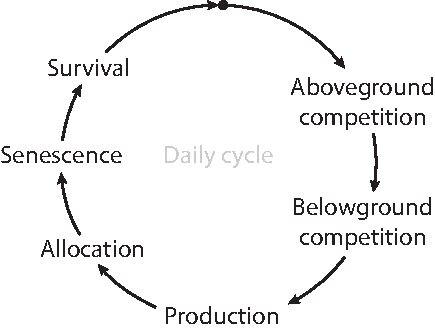
\includegraphics{./Figures/daily_cycle_t.pdf}
\caption{Processes in order during the daily cycle.}
\end{marginfigure}
\begin{itemize}
\setlength\itemsep{0em}
%\item \textit{resistance allocation}: the stored OM (in seeds or in storage tissues) are either invested in resistance molecules or in development;
%\item \textit{freezing}: frost damage on plants;
\item \textit{light competition}: the individual potential photosynthetic activity is computed based on average daily light and shoot properties;
\item \textit{water competition}: evaporation and the individual water update (and potential water uptake) are computed based on potential transpiration, water availability and potential evaporation;
\item \textit{production}: respiration and production are computed to give the net productivity in OM;
\item \textit{senescence}: based on lifespan a part of tissue is no longer active.
\item \textit{death}: death of individuals based on their age and their desiccation stage (number of consecutive days with negative growth).
\item \textit{allocation}: allocation of produced OM to the different carbon pools of the plant.
\textcolor{Gray}{\item \textit{grazing/cutting}: (optional) grazing or cutting of plants to a certain height. The grazing can be selective.}\footnote{remarks in \textcolor{Gray}{grey} are features or components implemented in the model but not used and-or calibrated.}
\end{itemize}


\section{Design concepts}

\subsection{Design concepts}
This part clarifies the rules that drive the dynamics of the model.

\paragraph{Emergence} 
The purpose of the model is to understand the rules that drive the community responses. We tried making the community dynamics emerge from the underlying processes of plant growth, resource use, and reproduction. That means that population dynamics are at least partially emergent from the surviving and reproducing individuals.
\textit{Partially} emergent because it depends on the invasion rules applied to the system. The traits and biomass distribution that describe the community are completely emergent from the individual traits exposed by the individuals and their relative biomass and abundance.
\begin{marginfigure}
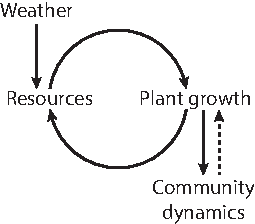
\includegraphics{./Figures/emergence.pdf}
\caption{Population dynamics emerging from plant growth and weather.}
\end{marginfigure}

\paragraph{Adaptation} Plants have in theory many options to adjust their phenotype and increase their fitness in response to changes in environmental conditions (resource availability, temperature, ...). High diversity of mountain grasslands suggests that multiple strategies coexist and that individuals do not change to converge toward a unique strategy. These strategies are set up at the species level by the species-specific traits (see table \ref{table:state_var_species}). Therefore, individuals may only adapt morphological traits but not strategic traits (unless there is an epigenetic mechanism added). These morphological traits are the relative biomass of shoot and root, the relative proportion of active and structural tissues in each leaf, and roots (controlling respectively the SLA and SRL and the overall resource acquisition cost)\footnote{and optionally the proportion of stored OM dedicated to frost resistance and not to growth}. Geometry traits (distribution of leaves and roots within space) are not considered plastic as grasses have far less control over their geometry than forbs or trees. Root distribution plasticity has been shown to greatly improve the individual and community productivity (Gemini article), but to keep the model (and implementation) simple we will ignore root distribution plasticity and foraging strategies to focus on allocation problems instead of spatial distribution questions. Shallow soils and relative small rooting zone are also arguments to ignore spatial distribution plasticity for roots.

\paragraph{Fitness}
\begin{marginfigure}
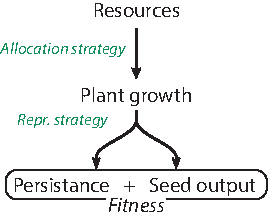
\includegraphics{./Figures/fitness.pdf}
\caption{Fitness emerges from the plant growth and the plant reproductive strategy.}
\begin{footnotesize}
The plant growth is the result of the interaction of the resource levels, the plant strategy, and the competitors.
\end{footnotesize}
\end{marginfigure}
In the model, the realised fitness can be estimated as the capacity of plants to maintain themselves or their descendants through time. It emerges from the productivity, allocation to storage or reproductive carbon pools, and survival. Assessing fitness as the average number of persistent individuals is, however, a bit hazardous in simulations limited in time and to a relatively small spatial scale. Plus, plants cannot easily make a prediction of such variable to adjust their phenotype. They need a proxy function for fitness that integrates measures of external conditions to evaluate the best strategy to develop. As said above, this strategy should be a composite between the species strategy and individual adjustment specific to the individual experience of the environment. Plant fitness is estimated by individual plant thanks to a gain function integrating current phenotype, species strategy, and projection of future conditions. This gain function can take multiple forms and be more or less constraint. In the context of the model, the function should include a measure of productivity that relies on the principle of functional equilibrium - that is the allocation of organic matter to maintain the balance between the shoot activity (transpiration) and root activity (water uptake). This equilibrium can be achieved by changes in shoot:root ratio only, or also changes in active over structural tissues ratio. Further details about the gain function are discussed in the dedicated paragraphs (\ref{par:allocation}). A more complex form of functional equilibrium incorporating nutrients (like nitrogen) could be added to the framework of this model.

\paragraph{Prediction} Adaptation or plasticity mechanisms imply that agents have an insight of what will be the future. In \model we consider that plants have two main sources of information. The first source of information is the genetic information. Indeed, the evolutionary process of genotype selection has led to the selection of genotypes adapted to the local conditions. This selection relationship can be seen as a link between environmental conditions and genetic information. Because plants cannot fully predict future environmental conditions, they grow following (at least partially) the plan contained in genetic information that match conditions where previous generations grew in.  This is an internal \textit{a priori} information about the external conditions. If the conditions where the seed grows change from the conditions its genotype has been selected for, the genetic information does not fit the environmental conditions is not sufficient enough to build a working phenotype. In this case, if the plant has a plasticity capacity, it can integrate the second source of information, in the form of the experienced conditions, to its "a priori" and forge a new estimation of what conditions will be. One question emerges to this idea is: how to create an image of future conditions and how to balance the genetic \textit{a priori} information with the experienced information? This balance can be described by a term of "reactivity" that describes the relative weight of genetic and experienced information. A reactive species will give a higher weight to experienced condition information, whereas a stable species will give a higher weight to genetic information.\\
\indent The way the two source of information are brought together and used to define the plant phenotype is at the core of plant strategy and is the main feature of the model \model.
\begin{figure}
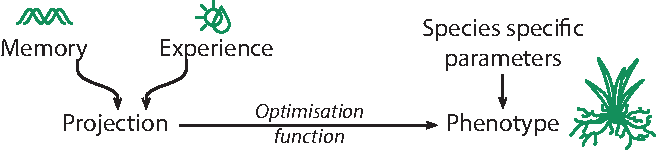
\includegraphics{./Figures/memory2phenotype_t.pdf}
\caption{Genetic and perceived information are both considered to determine the phenotype.}
\end{figure}
%\indent From that mechanism we can define two terms: the \textbf{climatic niche center} of a species is the \textit{a priori} information on climatic conditions, and the \textbf{plastic capacity} of a species is both its reactivity and its capacity to overcome the plasticity cost and invest in required tissues.
%Individuals do not estimate directly their fitness. They have however a way of estimating how well they perform depending on the level of resources they estimate. This measure is essential in plasticity mechanism as it drives plasticity. This measure is dependent on the plasticity mechanism chosen. Indeed plasticity can be approached in different ways that are discussed later, one mechanism consists in maintaining the \textit{functional equilibrium}, in this case, the fitness information is approached by the relative balance between above-and below-ground activities. The other mechanism is the \textit{optimisation}, that implies a more complex estimation of productivity, respiration, tissue turn-over and death changes and gives a more detailed approximation of individual fitness.
%\paragraph{Prediction and adaptation} As explained above, the "incomplete fitness proxies" used in the plasticity mechanisms require estimation of above- and below-ground activities, based on their trait values (SLA and SRL) and on an estimation of future external conditions (temperature, water availability and light availability). The originality of our approach is to make this estimation depending on both species-specific parameters and individual experience. The conditions are estimated as the weighted mean between the species-specific genetic \textit{a priori} on resource availability and the potential resource availability normalized over exchange area. This makes the estimation by one individual depending both on the species-specific "environmental niche" and the competition effects on resources. Moreover, this mechanism, because it includes relative weight to the two sources of information, allow multiple strategies for the estimation of external conditions and so on how to cope with resource levels variation.
%
%\paragraph{Adaptation} Adaptation is central in the model as we believe it explains a lot of intra-specific variability in mountain grassland ecosystems (cite Albert and others)
\section{Details}

Further details on daily mechanisms are described in the following paragraphs.


\begin{marginfigure}
%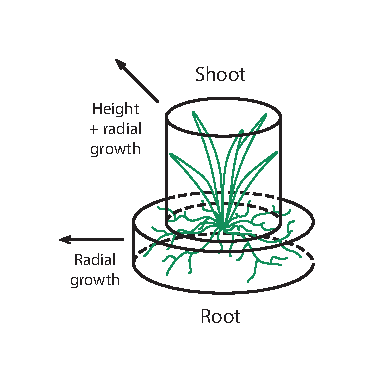
\includegraphics{./Figures/plant_geometry_m.pdf}
\caption{Overview of the model inputs and outputs.}
\end{marginfigure}

\subsection{Initialisation}
The model doesn't need particular initialisation if the state of the community species pool, the seedbank, and the soil are given as inputs. Otherwise, a set of \textit{E(n/s)} individuals are created from a set of \textit{s} species (randomly generated if not given) and randomly positioned on the soil grid, where \textit{s} and \textit{n} are respectively the number of species and the approximate number of individuals within the grid. Soil grid is also randomly generated within default ranges for critical and saturation water contents then slightly smooth, and homogeneously filled ($filling = \frac{w_{cont} - w_{crit}}{w_{sat} - w_{crit}}$).
 
\subsection{Inputs}
\model needs system state information (individuals, species, seed-bank and soil) and climate data. If the state of the system is not completely given, then the complete state is generated in the initialisation. The daily climate data at must contain the following fields:
\begin{itemize}
\setlength\itemsep{0em}
\item \textit{date};
\item \textit{radiance}, in $Watt.m^{2}$;
\item \textit{precipitation}, in mm;
\item \textit{mean temperature}, in K;
\item \textit{mean day temperature}, in K;
\item \textit{min temperature}, in K;
\item \textit{max temperature}, in K;
\item \textit{relative humidity} in \%;
\end{itemize}
Vapour pressure deficit is then computed from temperature and relative humidity.\\
\indent The climate data must explicitly differentiate the seasons (delimited by the first day of the year without snow and by the first day of the second semester with snow).

\subsection{Submodels}\label{subsection:submodels}

\paragraph{Germination} Individuals from the seed-bank randomly germinate according to their species-specific germination rate. Germination consist of investing a percentage ($mob$ parameter) of the seed mass into shoot and root biomass according to default traits. This is coupled with a round of random seed death following uniform law of parameter $seed_{surv}$. Living non germinating seeds stay in the seed-bank until the next season.\\
%
%\vspace{0.5em}
%\paragraph{Freezing resistance allocation} Resistance mechanisms are important for plants to invade harsh environments with perturbations such as grazing of frost events. Investment in free organic compounds is shown to provide resistance to frost. The concentration of such compounds is time variable and closely related to temperature. Other mechanisms morphological, structural, physiological can also play a role in frost resistance. For the sake of simplicity we will limit this aspect to the investment in circulating agents. Moreover, this aspect is crucial, indeed  because the frost risk is high at the beginning of the season, the choice of investing in resistance molecules instead of growing tissues is a strategy choice. Species can then be differentiated on a earlier growing/high frost risk - late growing/low frost risk axis, depending on their estimation of minimal temperature. Minimal temperature is estimated the same way other resources levels. Available stored biomass is invested in frost resistance is the estimated mean temperature is below 3\celsius .\\
%
% 
%\paragraph{Freezing} The freezing damages are calculated based on the concentration of organic matter dedicated to frost resistance is the plant. The LT50 (temperature at which 50\% of biomass is lost) is proportional to the concentration of resistance molecules compare to overall biomass. Daily leaf biomass lost due to frost is computed as follow:
%
%
%\begin{align}
%k_{frost} &= log(1/dam_{-1} - 1)/(-1 - LT_{50})\\
%dam &= \frac{1}{1 + e^{k_{frost}(T_{min} - LT_{50})}}
%\end{align}

\textbf{Daily processes}

\paragraph{Light competition}Light competition is central to all vegetation model as it constrains the photosynthetic activity and so plant growth. To avoid costly calculation of ray propagation we assume vertical homogeneous top radiation. Relief and orientation effects are taken into account in the computation of irradiance data.\\
Light competition sub-model allows calculation of individual potential photosynthesis activity and light at soil surface for evaporation calculation.\\
Competition for light is calculated independently for each pixel, potential photosynthetic activity is then aggregated at the individual level. Each pixel can be seen as a column of homogeneous layers containing at least one individual (top layer). For each layer, the light transmission is computed based on leaf density.


\begin{marginfigure}
\begin{tikzpicture}
\begin{axis}[marginplot,
legend style
={at={(1, 1.1)},
anchor=south east,
draw = none},
samples = 40,
%restrict y to domain=-300:700,
ylabel = $I_{h}$,
xlabel = $h$
%extra x ticks={0.618},
%extra x tick style={grid=major}
]

\addplot[black][domain = 0:10 ] {120 * exp(-1*x)};
%\addplot[gray][domain = 0:1 ] {(1/(0.022 * 1)) * ((1/0.05 - 1)*x) - %(7*exp(7*x) + 0.03)};
%\legend{$I_{h}$}
\end{axis}
\end{tikzpicture}
\label{fig:derivaives}
\caption{Net gain function and its first derivative.} Looks like there is some kind of mismatch here.
\end{marginfigure}

\begin{equation}\label{eq:Ih}
I(h) =  I_{0} e^{-LAI(h)}
\end{equation}

where $LAI(h)$ is the cumulative LAI at the bottom of layer \textit{l} (between $h$ and $h+\Delta_{h}$) defined as the homogeneous layer delimited by the top of consecutive individuals in the same pixel. The LAI is calculated like this:
\begin{equation}\label{eq:LAI}
LAI(h) = LAI(h+\Delta_{h}) +   \Delta_{h} . pix\_width^{2} \sum_{i\ in\ l}d_{i}.coverage_{i, p}
\end{equation}
where $d_{i}$ is the individual leaf area density corrected by the coverage ($0< coverage =< 1$) of the pixel $p$ by the plant $i$, $\Delta_{h} = (h_{l} - h_{l-1})$ is the height of the layer $l$.\\
Following Thornley and Johnson, the potential photosynthetic leaf activity is calculated as:


\begin{marginfigure}
\begin{tikzpicture}
\begin{axis}[marginplot,
legend style
={at={(1, 1.1)},
anchor=south east,
draw = none},
samples = 1000,
%restrict y to domain=-300:700,
xlabel = $I (W.cm^{2})$,
ylabel = $P_{leaf} (gCO_{2}.cm^{-2}s^{-1}) check that$
%extra x ticks={0.618},
%extra x tick style={grid=major}
]

\addplot[black][domain = 0:0.04 ] {(\paralpha * x * \parPmax ) /(\paralpha * x + \parPmax ) };
\legend{}
\end{axis}
\end{tikzpicture}
\label{fig:derivaives}
\caption{Photosynthetic saturation function}
\end{marginfigure}

\begin{equation}\label{eq:Pleaf}
P_{leaf}(h) = \frac{\alpha. I_{leaf}(h).P_{max}}{\alpha I_{leaf}(h)+P_{max}}
\end{equation}
where $I_{leaf}(h)$ is the light absorbed by the leaf at height $h$, $\alpha$ the initial slope of the light response curve and $Pm_{i}$ the maximum photosynthetic rate per unit of area and unit of time.
% where $I_{leaf}$ is the light absorbed by the leaf and the photosynthetic potential rate $Pm_{i}$ is linearly related to active biomass per leaf area as follow:
%\begin{equation}
%Pm_{i} = min(P_{slope} \frac{Leaf_{Act_{i}}}{Area_{i}}, P_{max})
%\end{equation}
$I_{leaf}$ is the radiance at the leaf surface, derived by correcting the radiance at the top of the layer following the equation used in Taubert with the extinction and transmission coefficients $k$ and $m$:

\begin{equation}
I{leaf}(h) = \frac{k}{1-m}I(h)
\end{equation}

The equation \eqref{eq:Pleaf} can be integrated over the leaf surface by mixing it with equations \eqref{eq:Ih} and \eqref{eq:LAI} to give the total potential photosynthesis for layer $l$ in pixel $p$:
\begin{equation}\label{Ppixlay}
P_{leaf}(p,l) = d_{i}.coverage_{i, p}.\Delta_{h}(l)\int_{h_{bottom}}^{h_{top}}P_{leaf}(h)
\end{equation}
%
%\begin{equation}
%P_{leaf}(l) = \int_{h_{l-1}}^{h_{l}}P_{leaf}.dLeaf = Leaf_{area}\left[- Pm_{leaf}.log(|m.Pm_{leaf} - Pm_{leaf} - \alpha.I_{h(leaf)}|)\right]_{h_{l}}^{h_{l-1}}
%\end{equation}

the total leaf potential photosynthesis is then calculated as follow:
\begin{equation}\label{eq:PS_pot}
PS_{pot} = \sum_{p\ in\ shoot}\sum_{l\ in\ pixel}P_{leaf}(p,l)
\end{equation}
\indent Potential photosynthesis must then be converted to potential transpiration to define the water demand. The conversion from photosynthesis to transpiration is done by dividing the potential photosynthesis by the water use efficiency ($WUE$). The potential activity of leaves are also dependent on the regulation of stomata so the transpiration can be written:
\begin{equation}
transp = \frac{PS_{pot} . g_{red}}{WUE}
\end{equation}

\textcolor{Gray}{\paragraph{Stomatal regulation} Photosynthesis depends on gazes exchanges at the leaf surface. These fluxes result from relative concentration in carbon dioxide and water, and from the stomatal conductance. Stomatal conductance is reduced and limits productivity when vapour pressure deficit is too high \sidenote{$g_{red}$ is set to 1 for current version to avoid potential problems between allocation and regulation}. A linear relationship describe this relationship:
\begin{equation}
g_{red} = 1+ VPD_{g\_red}
\end{equation}}

\paragraph{Evaporation} Potential evaporation is calculated for each pixel depending on the light at soil surface:

\begin{marginfigure}
\begin{tikzpicture}
\begin{axis}[marginplot,
legend style
={at={(1, 1.1)},
anchor=south east,
draw = none},
samples = 1000,
%restrict y to domain=-300:700,
ylabel = $\beta$,
xlabel = $\theta$,
extra x ticks={0.8},
extra x tick style={grid=major}
]

\addplot[black][domain = 0:0.8 ] {(1/4) * (1-cos(deg(x/0.8 * pi)))^2};
\addplot[black][domain = 0.8:1 ] {1};
%\legend{$I_{h}$}
\end{axis}
\end{tikzpicture}
\label{fig:derivaives}
\caption{Evaporation  limitation function.}
\end{marginfigure}

\begin{align}
 \beta &= 0.25 * (1 - cos(\frac{\theta}{\theta_{sat}} * \pi))^{2} & if water_{cont} \le water_{sat}\\
 \beta &= 1 & otherwise\\
 PET &= 0.0023. \sqrt{(T_{max} - T_{min})} * (T_{mean} + 17.8)\\
 evap &= PET . \beta . I_{surface} . daylength
\end{align}

\paragraph{Water competition} Water competition is also computed at the pixel level. To determine the water uptake, first the individual water demand is computed as the minimum between the transpiration and the potential water uptake. Transpiration demand per pixel is easily calculated by dividing the total potential transpiration by the volume in the pixel $V_{i,p}$ over the overall root volume $V_{i}$. Water potential uptake is the product of root area in the pixel and root water uptake rate reduced by the water availability reduction factor $U_{lim}$, leading to the water demand for individual $i$ in pixel $p$:
\begin{align}
transp_{i}(p) &= transp . \frac{V_{i,p}}{V_{i}}\\
Wpot_{i}(p) &= Root_{area}(p).U_{max}.U_{lim}\\
Wdem_{i}(p) &= min(transp_{i}(p), Wpot_{i}(p))\\
\end{align}
where, the limitation function $U_{lim}$ is defined as in \parencite{reineking_environmental_2006}:

\begin{marginfigure}[-40pt]
\begin{tikzpicture}
\begin{axis}[marginplot,
legend style
={at={(1, 1.1)},
anchor=south east,
draw = none},
samples = 100,
%restrict y to domain=-300:700,
xlabel = $\theta$,
ylabel = $U_{lim}$
%extra x ticks={0.618},
%extra x tick style={grid=major}
]

\addplot[black][domain = 0.21:0.99 ] {exp(\parbetazero * (1/(1-0.2) - 1/(x-0.2))) };
%\legend{Water limitation}
\end{axis}
\end{tikzpicture}
\label{fig:derivaives}
\caption{Water uptake limitation response function to soil saturation}
\end{marginfigure}

\begin{align}
U_{lim} &= exp\left(\beta_{\theta} \left( \frac{1}{\theta_{s} - \theta_{crit}} - \frac{1}{\theta - \theta_{crit}}\right)\right) & if \theta < \theta_{crit}\\
 &= 0 & otherwise
\end{align}

%Where $U_{i}$ is related to the maximum water uptake $U_{max}$ and to the the $\frac{Root_{Act_{i}}}{Area_{i}}$ as in equation \eqref{eq:Pleaf}.\\
The total water demand per pixel is then the sum of all individual water demand of the pixel and potential evaporation. If the total water demand exceeds the total water availability ($W_{av}$ product of water content and soil volume in the pixel) then the available water is distributed proportionally to the individual demand.\\
\begin{equation}\label{eq:water_uptake}
Wup_{i} = Wdem_{i} . \frac{Wdem_{total}}{min(Wdem_{total}, W_{av})}
\end{equation}


\indent The potential water uptake ($Wpup$), non limited by the transpiration is calculated the same way but considering $Wdem_{i} = Wpot_{i}$ in equation (\ref{eq:water_uptake}).\\
\indent Because the water competition is computed at the pixel level, there is no compensation between two pixels containing respectively not enough and too much water.\\
\indent No radial flow of water between pixel is implemented in the model. This simplification leads inevitably to edge effects, but allows simpler implementation and is partially covered by the effect of the pixel size. Indeed, increasing pixel size would have similar effect in the pixels at the border of the rooting zone than radial flow because it would increase the potential water pool plant has access to.\\

\indent Once potential and realised transpiration and water uptake are computed, 
plant productivity can be calculated.


\paragraph{Production, and respiration} Following previous vegetation models, the respiration is decomposed in growth respiration and maintenance respiration. The first is function of trait values, biomass and temperature:
\begin{equation}
R_{m} = \left(R_{act}.\left(Act_{ag} + Act_{bg}\right)\right) . daylength . T_{effect}
\end{equation}
where $R_{act}$ is the respiration rate of active tissues, and $Act_{ag}$ and $Act_{bg}$ are the active biomass pools in shoot and root.\\
\indent Net Primary production (in $CO_{2}$ equivalent) can then be calculated the difference of GPP and respiration, then converted in OM production thanks to tissue carbon content (under the assumption of fixed carbon content for leaf and roots between species):
 \begin{align}
 NPP_{carbon} &= (1- R_{g}) . (WUE . min(w_up, trans_p) - R_{m}) - BM_{total} * Pl_cost\\
 NPP_{OM} &= NPP_{carbon} . (12/44) / TCC
\end{align} 
Here $R_{g}$ is a fixed parameter but is set to $0$ if the difference between gross productivity ($GPP = WUE . min(w_up, trans_p) - R_{m}$) and maintenance respiration is negative. $Pl_{cost}$ is the plasticity cost as calculated in the dedicated paragraph below.

\paragraph{Temperature effect} Temperature has a effect of plant activity, this effect can be modelled by a bell shape function around an optimum value of 20 \celsius . See Lohier for details.


\paragraph{Condition estimation} The projection of environmental conditions is central in any implementaion of phenotype plasticity. Differences between the current perception of environment and the projections lead to adjustment of phenotype to increase fitness. In the model \model this projection results from hte averaging of two key concept: memory and perception. The latter is relatively simple to understand and corresponds to the perceived resource availability computed as the mean potential exchange rate per unit of area (total leaf or root area) and per hour(the hourly measure is used instead of daily measure to simulate the ability of plant to perceive the photoperiod. This is an easy way of taking into account one aspect of seasonality without complicating the model. However, it also reduce the range of memory and its impact to determine the phenotype, as an additional information would be needed to define the optimum phenotype: the day length).:
\begin{align}
light_{exp} &= \frac{transp}{exhange area_{ag}}\\
water_{exp} &= \frac{Wpup}{exchange area_{bg}}\\
\end{align}
The former is related to the species (or group) history and result from processes of selection and acclimation. It is the default projection of resource availability when the plant is not plastic. 
\begin{align}
light_{est}(t+1) &= (1 - \tau).light_{exp}(t) + \tau . light_{memory} . daylenght(t+1)\\
water_{est}(t+1) &= (1 - \tau).water_{exp}(t) + \tau . water_{memory} . daylenght(t+1)
\end{align}
\indent Because these are supposed to be expected conditions for the future, other formulation can be used instead of an average that is likely to introduce a lag in estimations. For example the following equation allow for a more stable projection that better fits the slower process of plant physiology adjustments:
\begin{align}\label{eq:projection_alt}
light_{est}(t+1) &= ((1 - \tau_{react}).light_{exp}(t) + \tau_{react} . light_{est}(t))((1 - \tau_{amp}) + \tau_{amp} . light_{memory}) . daylenght(t+1)
\end{align}
with $\tau_{amp}$ and $\tau_{react}$ being respectively amplitude and reactivity where only $\tau_{amp}$ is used in the first equation. Such solution could limit sensitivity and phenotypic instability. IN addition, such formulation would also better capture the accumulation of stress signals and would lead to a softer and more stable phenotypic shift.\\
\indent The estimation of external conditions as expressed here is then used to select the best allocation scheme during the allocation process. Limited here to levels of two resources (light and water), this estimation equation could be extended to other mechanisms such as herbivory risk, frost risk, humidity impact on water pressure deficit.\\

\paragraph{Allocation} \label{par:allocation}
Allocation is primordial in plant development and ontogeny. The following paragraph detail the implementation of the plastic allocation in \model.\\

\textbf{Maturity:} For most of plants the development cycle is divided in two phases of different durations: the vegetative phase when plant growths organs to gather resources and product OM, and the reproductive phase when plant take advantage of these organs to accumulate carbon and invest them in reproduction mechanisms. Plants are considered mature (they switch from vegetative to reproductive phase) in \model when the phenologic variable has reach a species specific threshold. The phenologic variable can be either the age, the height, the biomass, degree.days, in the current version total living biomass is used as trigger for reproductive phase.\\

\textbf{Allocation to supporting tissues:} Even-though grasses do not grow tall vegetative parts like trees, some grow vertically and they are exposed to stronger winds than most of forest. Therefore they need structural supports\sidenote{This supporting tissue mechanic is also needed to avoid exponential growth rate.}. Not all grasses grow stem, but they'll have stronger central vein in their leaves to structurally support the weight of leaves. In addition shoots and roots also need supporting tissues for water transport, for this reason the minimal mechanical support needed is calculated as a function of total living biomass:
\begin{equation}
support = \alpha . (BM_{ag} + BM_{bg})^\gamma
\end{equation}
where $\alpha$ and $\gamma$ are allometry coefficients.\\

\indent At each time step we must determine what fraction of new OM will be allocated to tissues growth while the remaining will support these need tissues. This leads to an optimisation problem numerically solved by the function \texttt{uniroot}.\\
%Despite the ambiguity in the name, there is a fundamental difference between structural tissues and supporting tissues: the former is part the individual organs and  
%\indent To avoid complex allocation optimisation problem, the allocation of supporting tissue is done before any other allocation. Is the support is not sufficient, no organic matter can be invested in vegetative development. The biomass the plant needs to invest in the stem is defined as:
%\begin{equation}
%\Delta_{stem} = max(support - (stem + Str_{ag}), 0)
%\end{equation}
%where $Str_{ag}$ is the structural biomass in shoot.\\
\begin{figure}
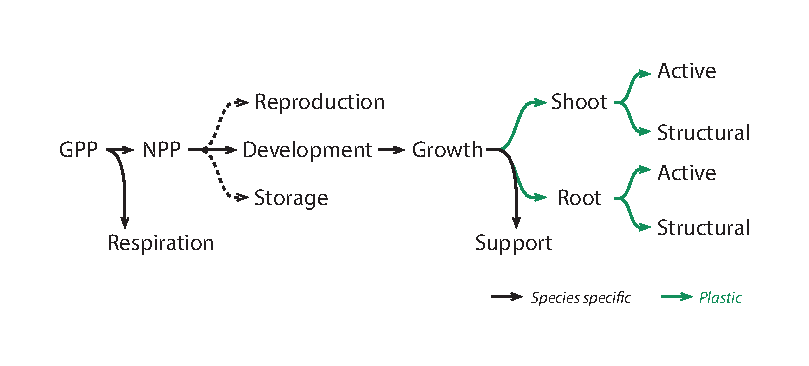
\includegraphics{./Figures/allocation_path_t.pdf}
\caption{Allocation of produced organic matter to different processes and pools.}
\end{figure}

\textbf{Allocation to organs:} Allocation of produced organic matter is central in vegetation as it shapes the plant and define the strength of the different organs. There are multiple ways to model the distribution of produced organic matter between the plant organs. We believe that such mechanism has great impact on individual development and response to external conditions, and so on community dynamics. To explore the role of this mechanism, multiple options are implemented. The different allocation algorithms are summarised in table \ref{table:alloc_algo}.\\
\indent There are two major components in the allocation algorithm:
\begin{itemize}
\item the objective function;
\item the plastic dimensions.
\end{itemize}
The \textit{objective function}: it is the function that give an fitness estimation or gain metrics for any given phenotype. This function is used to compute the optimum phenotype (phenotype at which the function is evaluated at the maximum value), or rank alternative phenotypes\sidenote{in this case, if not all possible phenotypes are tested, the solution might be only a local optimum. This is the case in \model.}. \\
The \textit{plastic dimensions}: they are the dimensions along which the individual can move. The space defined by these dimensions is the phenotypic space within which each individual plant can look for an alternative phenotype. They do not necessarily fully define a phenotype since some dimensions of the individual's phenotype can be fixed \sidenote{either by shared parameters of species specific ones.}. \\
\begin{figure}
\includegraphics{./Figures/strategy_space_algo.pdf}
\caption{Trajectories of a plant in the trait space depending on the plastic dimensions explored.}
\end{figure}
\indent The objective of this step of the model is to solve the objective function with the unknown variables being the plastic dimensions (RSR, SLA and SRL). In case of simple equations an analytical solution could be used to find an optimum \sidenote{under the condition that such optimum exists. The design of the model should ensure that.}. However, because the analytical solutions are already non trivial and the model is likely to evolve, a numeric solving method is adopted. \textbf{Need to detail the random algorithm.}\\
Also make a note on multiple optimum and the choice for a 'gradient descent" type of algorithm. Also sensitivity at eraly stages 

%TAble of plasticity mech
\begin{table*}
\caption{Allocation algorithms implemented in \model} 
\label{table:alloc_algo}
%\begin{center}%
\begin{tabular}{l|c|c c c}
Algorithm & Objective & variable RSR & variable SLA-SRL & stochastic \\ 
\hline 
No plasticty & $-$ & $\circ$ & $\circ$ & $\circ$ \\
Equilibrium & functional eq. & $\bullet$ & $\bullet$ & $\bullet$ \\
Eq-Fixed & functional eq. & $\bullet$ & $\circ$ & $\bullet$ \\
Optimisation & instantaneous gain & $\bullet$ & $\bullet$ & $\bullet$ \\
Optim-Fixed & instantaneous gain & $\bullet$ & $\circ$ & $\bullet$ \\
\end{tabular} 
%\end{center}
\vspace*{0.5cm}
\end{table*}

\textbf{No plasticity allocation:} this allocation is very similar to classic vegetation model where the biomass is allocated to the different carbon pools according to species specific parameters. But \model differs from other models by the order of the different steps of growth. In this model, the senescence comes between the allocation step and the resource competition-production steps \sidenote{see plastic allocation algorithm for explanation}. The partitioning coefficient are directly computed from species default trait to maintain the phenotype after senescence.

\textbf{Fixed trait allocation:} The fixed allocation supposes the allocation on OM to maintain trait values to fixed species specific values. The shoot:root ratio may however change to maintain functional equilibrium. The shoot root ratio is derived from the following equation of the functional equilibrium:
\begin{align}\label{eq:equilibrium}
SLA . BM_{ag} . light_{est} &= SRL . BM_{bg} . water_{est}\\
\frac{BM_{ab}}{BM_{bg}} &= \frac{SRL}{SLA} . \frac{water_{est}}{light_{est}}
\end{align}
where $light_{est}$ and $water_{est}$ are the estimated resource availabilities.
%
%\subparagraph{Plastic functional equilibrium} This allocation mechanism is also based on the functional equilibrium, however it incorporate changes in traits, that means that the proportion between active and structural tissues in an organ can change. This idea is supported by tha fact that plants change both their shoot:root and their trait values when conditions change. From a perspective with only one allocation dimension (shoot or root in "fixed trait allocation") with three dimensions (shoot or root, active or structural in shoot and in root tissues), the number of constraints must increase to find a unique solution. The functional equilibrium only is not sufficient to define the allocation scheme as multiple solutions satisfy this constraint. The solution is to chose among all possible allocation schemes the closest to the current allocation, the shortest path to functional equilibrium. This is done by minimising the 
% doesn't work for now

\textbf{Plastic trait allocation:} Another approach to allocation is to try to optimize phenotype based on a fitness proxy. This proxy can  be the sum of NPP, tissue turn-over loss and plasticity cost. But in a complex model like \model, plant performance is function of multiple aspects:\
\begin{itemize}
\item individual organ efficiency;
\item relative mass of each organ;
\item balance between organ water exchange activities.
\end{itemize}
And this could be extended to herbivory or frost risks. To take into account all these components, and take advantage of having all processes already made explicit by the implementation in the model, the daily processes of senescence and production are recalculated according to the \textbf{estimation of conditions} and the plant phenotype. This function is used to rank different alternative phenotypes (algorithm detailed below).

\textbf{Plastic trait equilibrium:} An alternative approach can be easily derived from the previous one and extend the principle of the first: the functional equilibrium with plastic traits. This approach consists in using the same algorithm as before but rank phenotypes with a function negatively correlated to the difference between estimated shoot and root activity. Such mechanism would nonetheless require the algorithm to look for close solutions within the allocation space to avoid convergence or drift from species strategy. Having non zero cost of plasticity in this approach should limit the drifting of the plant phenotype.

\textbf{Fixed trait optimisation:} This algorithm takes the idea of the optimisation algorithm but limits the plastic traits to the RSR ratio. If we can expect similar response than the fixed trait equilibrium if we suppose that the equilibrium is the main aspect of plant performance, global efficiency being considered in this case the result may vary.

\paragraph{Plastic algorithm}

Alternative phenotypes are computed from the actual phenotype and random uniform distribution of available organic matter to the main active and structural carbon pools of the plant.\sidenote{talk about the order senescence production, and the way exchange rates are computed.} ... This algorithm has the advantage of being relatively cheap compared to other optimization functions, however, its performances are variables and it is very sensitive to the number of samples used. As a consequence there is a trade-off between model stability and performance as a function of the number of samples (\textit{i.e.} alternative phenotypes) considered.
\begin{figure}
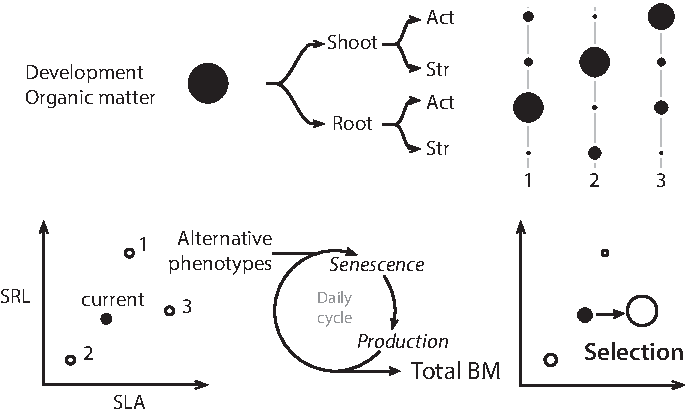
\includegraphics{./Figures/phenotype_ranking_t.pdf}
\caption{Algorithm for the evaluation and selection of randomly generated alternative phenotypes.}
\end{figure}

\paragraph{Plasticity cost}
The limits and costs of plasticity have long been discussed in the related literature. If \model is intended to be used to examine ecological costs and limits, it has to include physiological aspects of plasticity limits. There are two physiological processes involved in the mechanism of altering a phenotype based on changes in external conditions: sensing and signalling. 'Sensing' relates to the capacity of the individual to perceive environmental conditions. This is related to the capacity of the individual to perceive the environment and should, therefore, be considered constant over time. To take into account the cost of precise sensing, the first component of the plasticity cost is proportional to $\tau$.\\
The other component is related to the capacity of the plant to transmit this knowledge of conditions to change the development plan toward a new phenotype. This cost is proportional to the carbon-based distance (calculated as the difference between proportion of active tissues) between the default phenotype and the alternative (during allocation algorithm) or current phenotype.\sidenote{We could imagine cost based not on the default, but the previous phenotype, but it would have lead to large phenotypic shifting and convergence.}\\
Plasticity cost is the sum of both component and is proportional to the total biomass since most of the tissues should have the appropriated cell machinery and are affected b plasticity.
\begin{align}
pc_{maintenance} = (1 - tau) * pc_m \\
pc_{plasticity} = d_{traits} * pc_p
\end{align}
where $d_{traits}$ is the Euclidean distance between default phenotype and the alternative phenotype in the space defined by the proportion of active tissue for shoot and for roots.

\paragraph{Trait update}
Plasticity in trait suggests that trait values are modified in time. Because plants are described by single values (e.g. one SLA value for all leaves), this values must be updated after the plastic allocation. This values could be updated as the average of old tissue value weighted by old biomass and new tissue value weighted by the freshly produced biomass. This, however, would work only if active on structural tissues ratio linearly linked to others traits. This is not the case, it is then simpler to consider that organs have uniform active and structural distribution. This hypothesis suggests that whenever the allocation scheme change, old tissue reallocate their own biomass to follow the new scheme. Nevertheless, to avoid full plasticity allowed by this hypothesis, the changes in trait carbon pool sizes are limited by the produced biomass available for plant development.\\ollowing the following survival probabilities:


\indent From this, supposing homogeneous distribution of active and structural tissues within an organ allows to directly link the size of the carbon pools to average traits by the following relationships:
\begin{marginfigure}
\begin{tikzpicture}
\begin{axis}[marginplot,
legend style
={at={(1, 1.1)},
anchor=south east,
draw = none},
samples = 100,
%restrict y to domain=-300:700,
xlabel = $p_{act_{shoot}}$,
ylabel = $SLA$
%extra x ticks={0.618},
%extra x tick style={grid=major}
]

\addplot[black][domain = 0:1] {1/(\parth *  x * \parrhoas + \parth * (1 -  x) * \parrhoss * \parvts) };
%\legend{Water limitation}
\end{axis}
\end{tikzpicture}
\label{fig:SLA}
\caption{Specific Leaf Area as a function of the proportion in active tissues in shoot}
\end{marginfigure}

%  th_{a} &= \frac{\frac{act}{str}_{s} . th . \rho_{ss}}{\rho_{as} + \frac{act}{str}_{s} . \rho_{ss} }\\
%  s_{a} &= \frac{\frac{act}{str}_{r} . s_{root} . \rho_{sr} }{ \rho_{ar} + \frac{act}{str}_{r} . \rho_{sr}}\\
\begin{align}
  SLA &= \frac{1}{(th .  p_{act_{shoot}} . \rho_{as} + th . (1 -  p_{act_{shoot}}) . \rho_{ss} ) . V_{t}}\\
  SRL &= \frac{1}{(s_{r} .  p_{act_{shoot}} . \rho_{ar} + s_{r}.(1 -  p_{act_{shoot}}) . \rho_{sr}}
\end{align}


\paragraph{Senescence}

Senescence is the process of ageing of tissues. This process usually occurs at the scale of an individual organ (e.g. a leaf), however, \model does not consider organs independently because it would be complex and computationally expensive to follow multiple leaves and roots for all individuals. So the process is considered homogeneous over all tissues. To emulate the senescence process senescence is calculated from the tissues lifespan, giving :

\begin{marginfigure}
\begin{tikzpicture}
\begin{axis}[marginplot,
legend style
={at={(1, 1.1)},
anchor=south east,
draw = none},
samples = 500,
%restrict y to domain=0:1,
xlabel = $P_{act}$,
ylabel = $Lifespan (days)$
%extra x ticks={0.618},
%extra x tick style={grid=major}
]

\addplot[myGreen][domain = 0:0.99 ] {(\parlsszero * (1- x^\parlssone) ) };
\addplot[black][domain = 0:0.99 ] {(\parlsrzero * (1- x^\parlsrone) ) };
\legend{Aboveground, Belowground}
\end{axis}
\end{tikzpicture}
\label{fig:lifespan}
\caption{Lifespan of organs as a function of proportion of active tissues.}
\end{marginfigure}

\begin{align}
sen_{leaf} &= \frac{1}{LLS}\\
sen_{root} &= \frac{1}{RLS}
\end{align}

Because \model does not contain any mechanism preventing plant from growing only  active tissues\sidenote[][5pt]{it was intended to make the WUE negatively correlated to the amount of structural tissue per area.}, it is necessary for this cost function to make this strategy unreliable. The is then expressed as follow:

\begin{align}
LLS &= LSs_{s0} * (1- p_{act_{shoot}}^{LSs_{1}}) \\
RLS &= LSr_{s0} * (1- p_{act_{root}}^{LSr_{1}})
\end{align}


where $LLS$ and $RLS$ are respectively the leaf and the root lifespans calculated as negative log-linear relationships with the proportion of active tissue.\\
\indent Root senescent tissues disappear from the system. Information about senescent aboveground biomass is stored, but senescent biomass effect of light competition is ignored in this version because as it is implemented senescent tissues appear early in plant development and have large negative effect on light absorption.\\
\indent To the natural senescence and artificial cost of having only active tissue, an additional component can be added to the turn-over rate: the negative NPP. In case of negative NPP, the biomass will be taken from the already allocated following the shoot:root ratio. This can lead to a lower overall productivity (negative growth during unproductive periods) but also changes in the equilibrium if tissue have different efficiencies.\\

\paragraph{Death} Death is modelled as in Reineking \parencite{reineking_environmental_2006}. Age and desiccation (negative NPP) are the two reasons why a plant can die. The two death mechanism are simulated by independent random lotteries following the following survival probabilities:

\begin{marginfigure}[-10pt]
\begin{tikzpicture}
\begin{axis}[marginplot,
legend style
={at={(1, 1.1)},
anchor=south east,
draw = none},
samples = 100,
%restrict y to domain=-300:700,
xlabel = $age (days)$,
ylabel = $survival$
%extra x ticks={0.618},
%extra x tick style={grid=major}
]

\addplot[black][domain = 0:100] {exp(-((x/ \paralphaa)^\pargammaa- (max(x - 1, 0) / \paralphaa)^(\pargammaa)) ) };
%\legend{Water limitation}
\end{axis}
\end{tikzpicture}
\label{fig:derivaives}
\caption{Age related survival probability function}
\end{marginfigure}

\begin{align}
P_{d} &=  exp \left( - \left[\left(\frac{des}{\alpha_{d}}\right)^{\gamma_{d}} - \left(\frac{max(des - 1, 0)}{\alpha_{d}}\right)^{\gamma_{d}}\right]\right) & if NPP \le 0\\
&= 1 & otherwise\\
P_{a} &= exp \left( - \left[\left(\frac{age + 1}{\alpha_{a}}\right)^{\gamma_{a}} - \left(\frac{age}{\alpha_{a}}\right)^{\gamma_{a}}\right]\right)
\end{align}

State of dead individuals is store until the end of the season when seeds are stored in the seed bank. Seeds of dead individuals then join other seeds.

\paragraph{Reproduction \& persistence}
\textbf{Sexual \& clonal reproduction:} reproduction is handled at the end of the season. To limit the number of parameters reproduction is limited to the division of the invested biomass in reproduction by the species-specific seed biomass into a round number of seeds (the number of seed per plant could also be a differentiation axis). Clonal reproduction is not explicitly represented but can be mimic with bigger seeds and by adding a dispersion process around the parents. The seeds then are added to a potential seed-bank. This potential seed-bank is sampled, after eventual invasion, and merged with the existing seed-bank.\\
%\indent Control on the sampling process allows to model different type of ecosystems and test different hypothesises on invasions impact on community dynamics. The link between the community and the meta-community can also be explored through seed-bank control.\\
%\indent Three types of invasion/reproduction are currently implemented:
%\begin{itemize}
%\item closed environment reproduction: the seeds produced in the community return to the community, no invasion, the seed-bank size can be limited by a seed density limiting calculation explosions and simulating density mortality. Such mechanism should, in theory, lead to low diversity unless close equivalence between some species;
%\item constant reproduction in open environment: the seed-bank is generated at the meta-population levels, all species have the same biomass invested in reproductive pool independently from the local performance and seeds are randomly sampled. This mechanism stabilize greatly the system by does not allow to explore the meta-community dynamics and selection processes;
%\item productivity dependent reproduction in open environment: this mechanism is similar to the previous system but incorporates the productivity of the system by defining the seed input biomass as the total invested biomass in reproduction in the system at the end of the season. The system is stabilised but the overall productivity impacts the seed-bank dynamic.
%\end{itemize}

\textbf{Persistence} Some grasses are perennial and persist over the cold season. This is allowed in the model by investment in storage tissues instead of reproductive tissues.  At the end of the season, marked by the first snowfall, these plants (with non-null storage biomass) lose their living and supporting biomass, but will regrow from a large pool of store organic matter.

\textcolor{gray}{\paragraph{Grazing/cutting} Explore management effect on the community is one of the aims of the \model model. The management of mountain grassland will be explored only of the aspect of biomass removal, as productivity changes can be explored by changing the parameter values as the nutrients are not explicitly modelled. The management sub-model is not detailed here but it is based on the mapping of biomass and target trait (e.g. the fraction of structural biomass as a proxy for digestibility). Both cutting and grazing can be modelled but require management plan in the form of calendar of management operation and a cutting height or harvest objective.}\\

\section{Limitations and problems}

\subsection{Link to the real world and data}
The generalized framework introduced in \model allows to create a rich community in a high number of dimension strategy space, it, however, comes with downsides.\\
\indent One of the first problems is that some parameters (not explicitly detailed here) are hard to access (e.g. tissue density of active, or structural, tissue). It makes the calibration long as the incertitude for some parameters is very high. This is problematic when calibration is made difficult by a large execution time (see subsection below).\\
\indent Another issue with such model is that the high dimensionality of the species strategy space allows a lot of different strategies that are not viable. This could be overcome by selection mechanism over multiple plots, but again require a lot of simulation. Moreover, there are dependencies between viable strategies and parameter values that make it hard to restrict meta-community to viable species to set-up calibration runs.\\
\indent It is possible to extract summary statistics from the model output and compare them to information from collected data making calibration and community analysis easy. However going from the data to feed the model is harder, indeed without a great knowledge of a species it is hard to define its representation within the model framework. To do so would require the knowledge of the plasticity capacity to set the reactivity, anatomical traits to define default ratios of active over structural tissues, and climatic niche to define the \textit{a priori} estimation of external conditions. Without making a direct association with real species, it is possible and interesting to try to reproduce some strategies and explore their response to various conditions.

\subsection{Technical problems}

The model is implemented in \texttt{R} with some limiting function using \texttt{RCPP} to speed up the process. Simulations are fairly slow compare to theoretical \texttt{C++} equivalent code. The main problem is the choice of the data structure. Indeed agents are stored in data.frames that are often modified with the \verb|mutate| function, that makes the implementation much easier and the code readable, but slow down the execution due to constant condition checking on operations. This makes calibration routine methods almost impossible to use as they demand a very number of runs to be efficient.\\
\indent The slowness of the model also limit to simple algorithms for the research of favourable positions in the allocation space.
%\section{Model overview}
%\paragraph{pseudo-code and routine}
%\paragraph{allocation}
%mechanism and stochasticity\\
%5 types of allocation\\


%Take home message ####################################

%
%\subsection{Concepts}
%\paragraph{Memory} Genetic memory (see Sonia Sultan book for references). Selection and evolutionary processes.
%\paragraph{Equilibrium and efficiency}
%\paragraph{Optimum, strategy and memory} There might be optimum. But not easy to compute, especially when you consider more complex cost and interactions. Depend on different efficiencies and equilibrium... Also, you may want to avoid efficient by risky strategies (if you wrong, or if there is a quick shift). Need for strategic traits to drive allocation more than memory.\\
%Ok but what happen with optimisation allocation ? -> need the strategy to be tightly linked to memory. But that part has requirements: memory is a reliable source for strategy. Ultimately the resource availability is only one (ok, maybe two) dimension to phenotype optimisation. This strategy trait is necessary as other aspects of fitness are ignore (temperature implemented but not tested, grazzing vulnerability, frost damade, WUE, CO2 etc...) If you multiply mechanisms affecting the fitness you complexify the fitness landscape and allow for multiple strategies to be explored. Otherwise you must aartifically constraint. \\
%
%\indent \textbf{This is crucial to discuss this important aspect of strategic differenciation emerging for processes and how plant change strategy as the projection of environment evolves. Memory then plays more a role of sensitivity (with tau).}\\
%But for the moment the partial implementation of that through the artificial but meant to disappear default strategy is making analysis and assumptions difficult. Ok, but how do you treat it ? 
%
% equilibrium, resource use, resource availability, condition estimation
%\paragraph{Condition estimation}
%Important role of condition estimation. Perception mechanisms. (cost). Difference between plasticity and acclimation and epigenetics. 
%
%\subsection{Implementation}
%Why the use of a sampling method: complex effect of allocation and complex allocation system that is meant to be extended. Some results on the stability of phenotypes. How sampling method can drive the allocation.
%
%
%\section{Perturbations and resistances}
%
%\subsection{Climate}
%
%\subsection{Management}



%Take home message ####################################


%
%\subsection{comparison of different algorithms}
%full plasticity : freschet 2015 in poorter \& Ryser 2015
%the two sides of the performance/fitness: equilibrium and tissue efficiency\\
%age vs biomass.
%
%\section{Community dynamics parametrisation}
%Obj: demonstrate that the model is able to reproduce community dynamics (as it was designed for).\\
%Find parameters that allows coexistence (suggest plasticity should allow a diversity of strategy). SLA and height data. Phytosociology for 10m quadrats.
